\documentclass[t,aspectratio=169]{beamer} % 使用16:9宽高比
\usetheme{Madrid} % 选择Madrid主题
\usecolortheme{default} % 使用默认颜色主题

% 设置字体
\usepackage[UTF8]{ctex}
\usefonttheme{structurebold} % 加粗结构字体

% 数学包
\usepackage{amsmath, amssymb, bm}
\usepackage{url}
\usepackage{booktabs}

% 图形包
\usepackage{graphicx}

% 标题页信息
\title[9.2.权重衰减]{第9章：正则化}
\subtitle{第2节：权重衰减 (Weight Decay)}
\author{《深度学习基础》课程小组}
% \institute{上海立信会计金融学院}
\date{\today}

\begin{document}

% 标题页
\frame{\titlepage}

% 目录页
\begin{frame}
    \frametitle{目录}
    \tableofcontents
\end{frame}

% ============================================================
% 第一部分：权重衰减基础
% ============================================================
\section{权重衰减基础}

\begin{frame}
    \frametitle{1. 权重衰减：控制模型复杂度}
    \begin{itemize}
        \item 线性回归中引入正则化以\alert{控制模型复杂度}，作为限制参数数量的替代方案。
        \item 最简单的正则化项：\alert{模型参数的平方和}。
        \item 惩罚大数值的参数。
        \item 有效模型复杂度由\alert{正则化系数 $\lambda$} 的选择决定。
    \end{itemize}
\end{frame}

\begin{frame}
    \frametitle{1.1 概率视角：高斯先验}
    \begin{itemize}
        \item 加性正则化项可解释为\alert{权重向量 $\mathbf{w}$ 上零均值高斯先验}的负对数。
        \item 这提供了将先验知识纳入模型训练的\alert{概率视角}。
        \item \textbf{但问题在于}：
        \begin{itemize}
            \item 先验表达在\alert{模型参数}上。
            \item 领域知识更可能表达在\alert{从输入到输出的网络函数}上。
            \item 参数与网络函数的关系\alert{极其复杂}。
            \item 因此只有非常有限类型的先验知识能直接表达为参数先验。
        \end{itemize}
    \end{itemize}
\end{frame}

\begin{frame}
    \frametitle{1.2 为什么叫“权重衰减”？}
    \begin{itemize}
        \item 平方和正则化在机器学习文献中称为\alert{权重衰减}。
        \item 原因：在顺序学习算法中，它鼓励权重值\alert{向零衰减}，除非数据支持。
        \item \textbf{优点}：导数容易计算，便于梯度下降训练。
        \item 对于 (9.1) 形式的正则化项，梯度为：
        \begin{equation}
            \nabla \widetilde{E}(\mathbf{w}) = \nabla E(\mathbf{w}) + \lambda \mathbf{w}
            \tag{9.5}
        \end{equation}
        \item 注意：$1/2$ 因子在求导时消失（常被约定包含）。
    \end{itemize}
\end{frame}

\begin{frame}
    \frametitle{1.3 几何效果：收缩权重}
    \begin{itemize}
        \item 考虑二维参数空间 + 二次无正则化误差函数（图 9.3）。
        \item 坐标轴旋转以对齐\alert{海森矩阵的特征向量}。
        \item 正则化项的效果：\alert{收缩权重参数的幅度}。
        \item \textbf{关键观察}：对不同参数效果差异很大。
        \begin{itemize}
            \item $w_1$：输出对其相对不敏感 $\Rightarrow$ 正则化将其推向零。
            \item $w_2$：输出对其更敏感 $\Rightarrow$ 正则化影响较小。
        \end{itemize}
        \item \alert{有效参数数量}：正则化后仍保持“活跃”的参数数量。
        \item $\lambda \to \infty$：所有参数被驱动为零，有效参数数量为 0。
        \item $\lambda = 0$：有效参数数量等于模型总参数数量。
    \end{itemize}
\end{frame}

\begin{frame}
    \frametitle{1.4 误差函数等高线示意图}
    \begin{figure}
        \centering
        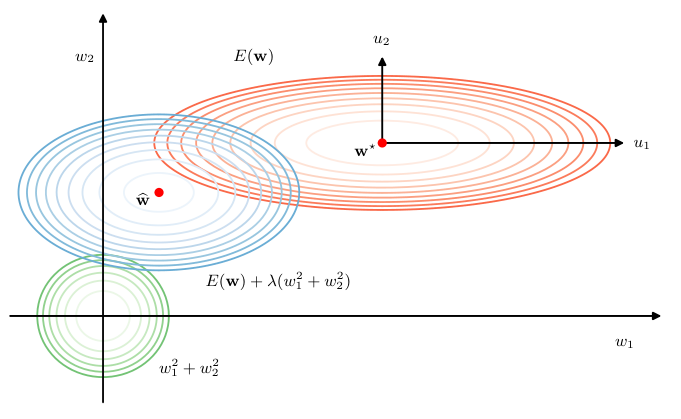
\includegraphics[width=0.30\textwidth]{fig-9-3.png}
        \caption{误差函数（红）、正则化项（绿）及其线性组合（蓝）的等高线。}
    \end{figure}
    \begin{itemize}
        \item $\lambda = 0$：最小误差在 $w^*$。
        \item $\lambda > 0$：正则化误差的最小值\alert{向原点偏移}。
        \item 偏移在 $w_1$ 方向更大（误差对其不敏感）。
        \item 正则化有效\alert{抑制对预测精度影响小的参数}。
    \end{itemize}
\end{frame}

% ============================================================
% 第二部分：一致性正则化
% ============================================================
\section{一致性正则化}

\begin{frame}
    \frametitle{2. 简单权重衰减的局限性}
    \begin{itemize}
        \item 简单权重衰减 (9.1) 破坏了网络映射的某些\alert{理想变换性质}。
        \item 考虑两层 MLP，线性输出单元。
    \end{itemize}
    \begin{block}{输入线性变换}
        对输入做线性变换：
        \begin{equation}
            x_i \to \widetilde{x}_i = a x_i + b
            \tag{9.8}
        \end{equation}
        可通过对应变换隐藏层权重保持网络映射不变：
        \begin{align}
            w_{ji} &\to \widetilde{w}_{ji} = \frac{1}{a} w_{ji} \tag{9.9} \\
            w_{j0} &\to \widetilde{w}_{j0} = w_{j0} - \frac{b}{a} \sum_i w_{ji} \tag{9.10}
        \end{align}
    \end{block}
\end{frame}

\begin{frame}
    \frametitle{2.1 输出变换与一致性要求}
    \begin{block}{输出线性变换}
        对输出做线性变换：
        \begin{equation}
            y_k \to \widetilde{y}_k = c y_k + d
            \tag{9.11}
        \end{equation}
        可通过变换第二层权重和偏置实现：
        \begin{align}
            w_{kj} &\to \widetilde{w}_{kj} = c w_{kj} \tag{9.12} \\
            w_{k0} &\to \widetilde{w}_{k0} = c w_{k0} + d \tag{9.13}
        \end{align}
    \end{block}
    \begin{itemize}
        \item \alert{一致性要求}：用原始数据和变换后数据训练的网络应等价，仅权重差一个线性变换。
        \item 任何正则化项都应与该性质\alert{一致}，否则会任意偏向某个等价解。
        \item 简单权重衰减 (9.1) 对所有权重和偏置\alert{一视同仁}，\alert{不满足}该性质。
    \end{itemize}
\end{frame}

\begin{frame}[allowframebreaks]
    \frametitle{2.2 一致性正则化项}
    寻找在线性变换 (9.9)(9.10)(9.12)(9.13) 下\alert{不变}的正则化项：
    \begin{equation}
        \frac{\lambda_1}{2} \sum_{w \in \mathcal{W}_1} w^2 + \frac{\lambda_2}{2} \sum_{w \in \mathcal{W}_2} w^2
        \tag{9.14}
    \end{equation}
    \begin{itemize}
        \item $\mathcal{W}_1$：第一层权重集合；$\mathcal{W}_2$：第二层权重集合。
        \item \alert{偏置被排除}在求和之外。
        \item 若重新缩放正则化参数 $\lambda_1 \to a^{1/2} \lambda_1$ 和 $\lambda_2 \to c^{-1/2} \lambda_2$，该正则化项保持不变。
    \end{itemize}
    \begin{block}{对应的先验分布}
        \begin{equation}
            p(\mathbf{w} \mid \alpha_1, \alpha_2) \propto \exp\left( -\frac{\alpha_1}{2} \sum_{w \in \mathcal{W}_1} w^2 - \frac{\alpha_2}{2} \sum_{w \in \mathcal{W}_2} w^2 \right)
            \tag{9.15}
        \end{equation}
        \begin{itemize}
            \item 该先验是\alert{非正常}的（无法归一化），因为偏置参数无约束。
            \item 非正常先验给正则化系数选择和贝叶斯模型比较带来困难。
            \item 通常为偏置包含\alert{单独的先验}（破坏平移不变性），有自己的超参数。
        \end{itemize}
    \end{block}
\end{frame}

\begin{frame}
    \frametitle{2.3 四个超参数的效果}
    \begin{itemize}
        \item 先验由四个超参数控制：
        \begin{itemize}
            \item $\alpha_1^\mathrm{b}$：第一层偏置的精度
            \item $\alpha_1^\mathrm{w}$：第一层权重的精度
            \item $\alpha_2^\mathrm{b}$：第二层偏置的精度
            \item $\alpha_2^\mathrm{w}$：第二层权重的精度
        \end{itemize}
        \item 效果（图 9.4）：
        \begin{itemize}
            \item $\alpha_2^\mathrm{w}$：控制函数的\alert{垂直尺度}
            \item $\alpha_1^\mathrm{w}$：控制函数值变化的\alert{水平尺度}
            \item $\alpha_1^\mathrm{b}$：控制变化发生的\alert{水平范围}
            \item $\alpha_2^\mathrm{b}$：控制函数的\alert{垂直偏移范围}
        \end{itemize}
    \end{itemize}
\end{frame}

\begin{frame}
    \frametitle{2.4 推广：任意分组}
    更一般地，可将权重分为任意数量的组 $\mathcal{W}_k$：
    \begin{equation}
        \Omega(\mathbf{w}) = \frac{1}{2} \sum_k \alpha_k \|\mathbf{w}\|_k^2
        \tag{9.16}
    \end{equation}
    其中
    \begin{equation}
        \|\mathbf{w}\|_k^2 = \sum_{j \in \mathcal{W}_k} w_j^2
        \tag{9.17}
    \end{equation}
    \begin{itemize}
        \item 例如：多层网络中可为\alert{每一层使用不同的正则化项}。
    \end{itemize}
\end{frame}

% ============================================================
% 第三部分：广义权重衰减
% ============================================================
\section{广义权重衰减}

\begin{frame}
    \frametitle{3. 广义权重衰减}
    简单二次正则化的推广：
    \begin{equation}
        \Omega(\mathbf{w}) = \frac{\lambda}{2} \sum_{j=1}^M |w_j|^q
        \tag{9.18}
    \end{equation}
    \begin{itemize}
        \item $q = 2$：对应二次正则化 (9.1)。
        \item 图 9.5 展示了不同 $q$ 值的正则化函数等高线。
    \end{itemize}
    \begin{block}{Lasso ($q = 1$)}
        统计文献中称为\alert{lasso} (Tibshirani, 1996)。
        \begin{itemize}
            \item 对二次误差函数，若 $\lambda$ 足够大，某些系数 $w_j$ 被驱动为零。
            \item 导致\alert{稀疏模型}：对应基函数不起作用。
        \end{itemize}
    \end{block}
\end{frame}

\begin{frame}
    \frametitle{3.1 稀疏性的来源}
    最小化正则化误差函数：
    \begin{equation}
        E(\mathbf{w}) + \frac{\lambda}{2} \sum_{j=1}^M |w_j|^q
        \tag{9.19}
    \end{equation}
    等价于在约束下最小化无正则化误差函数：
    \begin{equation}
        \sum_{j=1}^M |w_j|^q \leqslant \eta
        \tag{9.20}
    \end{equation}
    \begin{itemize}
        \item 两种方法可通过\alert{拉格朗日乘子}关联。
        \item 稀疏性来源见图 9.6：约束下的误差函数最小值。
        \item $\lambda$ 增大 $\Rightarrow$ 更多参数被驱动为零。
        \item 对比：二次正则化保留两个权重参数均为非零值。
    \end{itemize}
\end{frame}

\begin{frame}
    \frametitle{3.2 正则化的作用与权衡}
    \begin{itemize}
        \item 正则化允许复杂模型在\alert{有限规模数据集}上训练而不严重过拟合。
        \item 本质：\alert{限制有效模型复杂度}。
        \item \textbf{但问题转移了}：
        \begin{itemize}
            \item 从“找到合适的可学习参数数量”
            \item 转变为“确定合适的正则化系数 $\lambda$ 值”
        \end{itemize}
        \item 模型复杂度问题将在下一节讨论。
    \end{itemize}
\end{frame}

% ============================================================
% 第四部分：总结
% ============================================================
\section{总结}

\begin{frame}
    \frametitle{4. 本节总结}
    \begin{itemize}
        \item \alert{权重衰减}：最简单的正则化项，模型参数平方和。
        \begin{itemize}
            \item 惩罚大数值参数，控制模型复杂度。
            \item 可解释为零均值高斯先验的负对数。
            \item 梯度容易计算：$\nabla \widetilde{E} = \nabla E + \lambda \mathbf{w}$。
        \end{itemize}
        \item \alert{几何效果}：收缩权重，对输出不敏感的参数被推向零。
        \item \alert{有效参数数量}：正则化后仍活跃的参数数量。
        \item \alert{一致性正则化}：
        \begin{itemize}
            \item 简单权重衰减破坏线性变换性质。
            \item 一致性正则化项应对权重缩放和偏置平移不变。
            \item 偏置应排除在求和之外，或使用单独先验。
        \end{itemize}
        \item \alert{广义权重衰减}：
        \begin{itemize}
            \item $\Omega(\mathbf{w}) = \frac{\lambda}{2} \sum |w_j|^q$
            \item $q = 1$：lasso，产生\alert{稀疏}模型
            \item $q = 2$：二次正则化
        \end{itemize}
        \item 正则化将模型复杂度问题\alert{转移}到正则化系数选择。
    \end{itemize}
\end{frame}

% ============================================================
% 第五部分：参考文献
% ============================================================
\section{参考文献}

\begin{frame}
    \frametitle{5. 参考文献}
    \begin{itemize}
        \item 教材：Bishop, C. M. \& Bishop, H. (2023). Deep Learning Foundations and Concepts. Springer Nature Switzerland AG.
        \item Tibshirani, R. (1996). Regression shrinkage and selection via the lasso.
        \item Bishop, C. M. (2006). Pattern Recognition and Machine Learning. Springer.
        \item Hastie, T., Tibshirani, R., \& Friedman, J. (2009). The Elements of Statistical Learning.
    \end{itemize}
\end{frame}

\end{document}